\documentclass[12pt,a4paper]{report}

% Essential Packages
\usepackage[utf8]{inputenc}
\usepackage[margin=1in]{geometry}
\usepackage{amsmath,amssymb,amsfonts}
\usepackage{graphicx}
\usepackage{booktabs}
\usepackage{tabularx}
\usepackage{listings}
\usepackage{xcolor}
\usepackage{hyperref}
\usepackage{cite}
\usepackage{fancyhdr}
\usepackage{titlesec}
\usepackage{setspace}
\usepackage{float}
\usepackage{needspace}
\usepackage{tikz}
\usetikzlibrary{calc, positioning}

\onehalfspacing

% Hyperref setup
\hypersetup{
    colorlinks=true,
    linkcolor=blue!70!black,
    citecolor=red!70!black,
    urlcolor=teal!70!black
}

% Code Listing Styling
\definecolor{codegreen}{rgb}{0,0.6,0}
\definecolor{codegray}{rgb}{0.5,0.5,0.5}
\definecolor{codepurple}{rgb}{0.58,0,0.82}
\definecolor{backcolour}{rgb}{0.96,0.96,0.96}

\lstdefinestyle{pythonstyle}{
    backgroundcolor=\color{backcolour},   
    commentstyle=\color{codegreen},
    keywordstyle=\color{magenta},
    numberstyle=\tiny\color{codegray},
    stringstyle=\color{codepurple},
    basicstyle=\ttfamily\footnotesize,
    breakatwhitespace=false,         
    breaklines=true,                 
    captionpos=b,                    
    keepspaces=true,                 
    columns=flexible,
    numbers=left,                    
    numbersep=6pt,                  
    showspaces=false,                
    showstringspaces=false,
    showtabs=false,                  
    tabsize=4,
    frame=single,
    rulecolor=\color{black!20},
    framesep=4pt,
    xleftmargin=12pt
}
\lstset{style=pythonstyle}

% Header and Footer
\pagestyle{fancy}
\setlength{\headheight}{15pt}
\fancyhf{}
\fancyhead[L]{\small Information Security Course Project}
\fancyhead[R]{\small TRAN HUU QUYET (066206014296)}
\fancyfoot[C]{\thepage}

\begin{document}

% -------------------------------------------------------------
% Title Page (100% English Academic Format with Official UTH Logo)
% -------------------------------------------------------------
\begin{titlepage}
    \thispagestyle{empty}
    \begin{tikzpicture}[remember picture, overlay]
        % Outer decorative border
        \draw[line width=1.5pt, color=blue!85!black] 
            ($(current page.north west) + (1.2cm,-1.2cm)$) 
            rectangle ($(current page.south east) + (-1.2cm,1.2cm)$);
        % Inner fine border (symmetrically inset by 1.35cm)
        \draw[line width=0.6pt, color=blue!85!black] 
            ($(current page.north west) + (1.35cm,-1.35cm)$) 
            rectangle ($(current page.south east) + (-1.35cm,1.35cm)$);
    \end{tikzpicture}
    
    \centering
    \begin{singlespace}
    \vspace*{-0.2cm}
    
    {\large \textbf{HO CHI MINH CITY UNIVERSITY OF TRANSPORT (UTH)}\par}
    \vspace{0.15cm}
    {\large \textbf{INSTITUTE OF INFORMATION TECHNOLOGY AND ELECTRICAL \& ELECTRONICS ENGINEERING}\par}
    
    \vspace{0.35cm}
    
\includegraphics[width=0.45\linewidth, height=1.7cm, keepaspectratio]{figures/logo_uth.png}\par
    \vspace{0.25cm}
    
    {\centering \rule{0.75\linewidth}{0.6pt}\par}
    \vspace{0.35cm}
    
    {\Large \textbf{COURSE PROJECT REPORT: INFORMATION SECURITY}\par}
    \vspace{0.15cm}
    {\textbf{Course Class ID:} \texttt{012012303303}\par}
    
    \vspace{0.6cm}
    {\normalsize \textbf{PROJECT TOPIC:}\par}
    \vspace{0.2cm}
    {\Large \bfseries STUDY AND IMPLEMENTATION OF MODERN CRYPTOGRAPHIC TECHNIQUES FROM FIRST PRINCIPLES\par}
    \vspace{0.2cm}
    {\large \textit{(AES-128, RSA, SHA-256, DSA)}\par}
    
    \vspace{0.8cm}
    \begin{minipage}{0.85\textwidth}
        \large
        \textbf{Instructor:} \quad \textbf{Dr. Tran The Vinh}\\[0.35cm]
        \textbf{Student Author:}\\[0.15cm]
        \begin{tabular}{|l|l|}
            \hline
            \textbf{Full Name} & \textbf{Student ID (SID)} \\
            \hline
            \textbf{Tran Huu Quyet} & \textbf{066206014296} \\
            \hline
        \end{tabular}
    \end{minipage}
    
    \vfill
    {\large \textbf{Ho Chi Minh City, November 2026}\par}
    \vspace*{0.2cm}
    \end{singlespace}
\end{titlepage}

\clearpage
\pagenumbering{roman}
\setcounter{page}{1}

% -------------------------------------------------------------
% Academic Integrity Statement
% -------------------------------------------------------------
\newpage
\chapter*{Statement of Academic Integrity}
\addcontentsline{toc}{chapter}{Statement of Academic Integrity}

I, \textbf{TRAN HUU QUYET} (Student ID: \textbf{066206014296}), hereby declare that:
\begin{enumerate}
    \item This course project report and its accompanying software implementation are entirely my own original work conducted independently in compliance with the academic integrity regulations.
    \item All cryptographic algorithms presented in this report---namely \textbf{AES-128}, \textbf{RSA}, \textbf{SHA-256}, and \textbf{DSA}---have been implemented in Python \emph{from first principles} without relying on any third-party cryptographic libraries (such as \texttt{cryptography}, \texttt{PyCryptodome}, \texttt{PyNaCl}, or OpenSSL).
    \item Artificial Intelligence and supplementary tools have been consulted strictly as assistive reference materials; all analyses, mathematical formulations, software implementations, and experimental verifications have been synthesized, verified, and substantively reviewed by myself.
    \item All external literature, standards (including NIST FIPS publications and RFCs), and intellectual sources have been duly acknowledged and cited in accordance with academic standards.
    \item I am fully prepared to defend, explain, and substantiate every aspect of the theoretical models and code routines submitted herewith before the instructor.
\end{enumerate}

\vspace{1.5cm}
\begin{flushright}
    \textit{Student Signature:}\\[0.5cm]
    \textbf{TRAN HUU QUYET}
\end{flushright}

% -------------------------------------------------------------
% Table of Contents & Lists
% -------------------------------------------------------------
\clearpage
\tableofcontents
\clearpage
\listoffigures
\clearpage
\listoftables

% -------------------------------------------------------------
% Chapters
% -------------------------------------------------------------
\clearpage
\pagenumbering{arabic}
\setcounter{page}{1}

\chapter{Symmetric-Key Cryptography: Advanced Encryption Standard (AES-128)}
\label{ch:aes}

\section{Historical Background, Development, and Design Motivation}
Prior to the adoption of the Advanced Encryption Standard (AES), the Data Encryption Standard (DES), formalized in 1977 as FIPS PUB 46, served as the dominant global standard for symmetric block encryption. However, the effective 56-bit key length of DES became critically vulnerable to exhaustive brute-force search attacks in the late 1990s (most notably demonstrated by the EFF DES Cracker ``Deep Crack'' in 1998, which broke DES in under 56 hours). Although Triple-DES (3DES) provided an interim extension by chaining three DES operations (yielding a 112-bit or 168-bit key), its $64$-bit block size raised severe concerns regarding birthday-bound collision attacks in high-throughput network environments (such as Sweet32). Furthermore, 3DES was computationally inefficient in software implementations due to DES's bit-oriented permutations designed originally for 1970s hardware.

In 1997, the National Institute of Standards and Technology (NIST) initiated an open, multi-year international competition to select a replacement. The criteria mandated:
\begin{enumerate}
    \item A symmetric block cipher supporting a fixed block size of 128 bits.
    \item Variable key sizes of 128, 192, and 256 bits.
    \item Strong cryptographic security margins against all known differential and linear cryptanalytic attacks.
    \item Computational efficiency, minimal memory footprints, and architectural versatility across 8-bit smart cards, 32-bit/64-bit microprocessors, and dedicated ASIC hardware.
\end{enumerate}
In October 2000, NIST selected the \emph{Rijndael} cipher, invented by Belgian cryptographers Joan Daemen and Vincent Rijmen, and formally standardized it as AES in FIPS PUB 197 \cite{fips197}. Unlike DES's Feistel network, AES utilizes a Substitution-Permutation Network (SPN), which processes all 128 bits in parallel in every round.

\section{Underlying Mathematical Foundations and Operating Principles}
The mathematical strength and efficiency of AES derive from algebraic operations defined over the Galois Field (finite field) of order $2^8$, denoted $\text{GF}(2^8)$ or $\mathbb{F}_{2^8}$ \cite{paarpelzl}.

\subsection{Finite Field $\text{GF}(2^8)$ Representation}
In AES, each byte $b = (b_7 b_6 b_5 b_4 b_3 b_2 b_1 b_0)_2$ is treated as a degree-7 polynomial with binary coefficients:
\begin{equation}
b(x) = \sum_{i=0}^7 b_i x^i = b_7 x^7 + b_6 x^6 + \dots + b_1 x + b_0 \quad \in \mathbb{Z}_2[x]
\end{equation}
Field addition is defined as polynomial addition modulo 2, equivalent to the bitwise XOR ($\oplus$) operator:
\begin{equation}
a(x) \oplus b(x) = \sum_{i=0}^7 (a_i \oplus b_i) x^i
\end{equation}
Multiplication is polynomial multiplication performed modulo an irreducible polynomial of degree 8. In FIPS 197, AES specifies the field polynomial:
\begin{equation}
m(x) = x^8 + x^4 + x^3 + x + 1 \quad (\text{hexadecimal: } \texttt{0x11B})
\end{equation}

\subsection{Multiplication by $x$ (\texttt{xtime}) and Galois Inversion}
Multiplication of a byte $b(x)$ by $x$ (hexadecimal \texttt{0x02}) corresponds to a left-shift by 1 bit, followed by a conditional XOR reduction with \texttt{0x1B} if the high-order bit $b_7 = 1$:
\begin{equation}
\texttt{xtime}(b) = 
\begin{cases} 
(b \ll 1), & \text{if } b_7 = 0 \\
(b \ll 1) \oplus \texttt{0x1B}, & \text{if } b_7 = 1
\end{cases} \pmod{2^8}
\end{equation}
Every non-zero byte $a \in \text{GF}(2^8)$ possesses a unique multiplicative inverse $a^{-1}$ satisfying $a \cdot a^{-1} \equiv 1 \pmod{m(x)}$. By Fermat's Little Theorem generalized to finite fields, $a^{2^8 - 1} \equiv 1$, hence $a^{-1} = a^{254}$.

\subsection{The Non-Linear S-Box Derivation}
The AES Substitution Box (S-Box) maps an input byte $a$ to an output byte $s$ via two algebraic steps:
\begin{enumerate}
    \item Compute the multiplicative inverse $b = a^{-1} \in \text{GF}(2^8)$, with the mapping $0^{-1} \triangleq 0$.
    \item Apply an affine transformation over $\text{GF}(2)$:
    \begin{equation}
    s_i = b_i \oplus b_{(i+4)\bmod 8} \oplus b_{(i+5)\bmod 8} \oplus b_{(i+6)\bmod 8} \oplus b_{(i+7)\bmod 8} \oplus c_i
    \end{equation}
    for $0 \le i < 8$, where $c = (01100011)_2 = \texttt{0x63}$.
\end{enumerate}
This algebraic formulation provides optimal resistance against differential and linear cryptanalysis while eliminating simple algebraic relationships between input and output.

\section{Complete Operational Procedure}
AES-128 operates on a 128-bit block viewed as a $4 \times 4$ column-major matrix of bytes, called the \emph{State}:
\begin{equation}
\text{State} = \begin{bmatrix}
s_{0,0} & s_{0,1} & s_{0,2} & s_{0,3} \\
s_{1,0} & s_{1,1} & s_{1,2} & s_{1,3} \\
s_{2,0} & s_{2,1} & s_{2,2} & s_{2,3} \\
s_{3,0} & s_{3,1} & s_{3,2} & s_{3,3}
\end{bmatrix}
\end{equation}
For a 128-bit key, AES executes $N_r = 10$ transformation rounds, as visually illustrated in Figure \ref{fig:aes_pipeline}.

\begin{figure}[htbp]
\centering
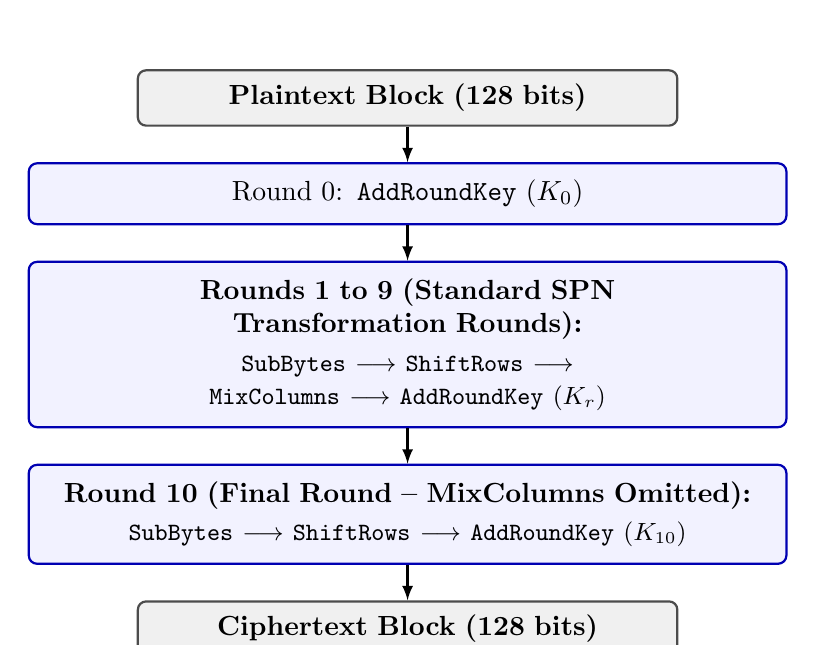
\begin{tikzpicture}[>=stealth,
    block/.style={rectangle, draw=blue!70!black, fill=blue!5, thick, text width=9.2cm, align=center, rounded corners=3pt, inner sep=6pt},
    io/.style={rectangle, draw=black!70, fill=gray!12, thick, text width=6.5cm, align=center, rounded corners=3pt, inner sep=5pt},
    line/.style={draw, -latex, thick}]
    
    \node (pt) [io] {\textbf{Plaintext Block (128 bits)}};
    \node (init) [block, below=0.45cm of pt] {Round 0: \texttt{AddRoundKey} ($K_0$)};
    \node (rounds) [block, below=0.45cm of init] {\textbf{Rounds 1 to 9 (Standard SPN Transformation Rounds):}\\
        \vspace{2pt}
        \small \texttt{SubBytes} $\longrightarrow$ \texttt{ShiftRows} $\longrightarrow$ \texttt{MixColumns} $\longrightarrow$ \texttt{AddRoundKey} ($K_r$)};
    \node (final) [block, below=0.45cm of rounds] {\textbf{Round 10 (Final Round -- MixColumns Omitted):}\\
        \vspace{2pt}
        \small \texttt{SubBytes} $\longrightarrow$ \texttt{ShiftRows} $\longrightarrow$ \texttt{AddRoundKey} ($K_{10}$)};
    \node (ct) [io, below=0.45cm of final] {\textbf{Ciphertext Block (128 bits)}};
    
    \path [line] (pt) -- (init);
    \path [line] (init) -- (rounds);
    \path [line] (rounds) -- (final);
    \path [line] (final) -- (ct);
\end{tikzpicture}
\caption{AES-128 Encryption State Pipeline and Transformation Architecture.}
\label{fig:aes_pipeline}
\end{figure}

\subsection{Key Expansion}
The 16-byte initial cipher key $K$ is expanded into an array of $4(N_r + 1) = 44$ words (32-bit each), denoted $W[0 \dots 43]$.
\begin{itemize}
    \item $W[0 \dots 3]$ correspond to the 4 columns of the initial key.
    \item For $i = 4, \dots, 43$:
    \begin{equation}
    \text{temp} = W[i-1]
    \end{equation}
    If $i \equiv 0 \pmod 4$:
    \begin{equation}
    \text{temp} = \text{SubWord}(\text{RotWord}(\text{temp})) \oplus \text{Rcon}[i/4]
    \end{equation}
    Then:
    \begin{equation}
    W[i] = W[i-4] \oplus \text{temp}
    \end{equation}
\end{itemize}
where $\text{RotWord}([a_0, a_1, a_2, a_3]) = [a_1, a_2, a_3, a_0]$, $\text{SubWord}$ maps each byte through the S-box, and $\text{Rcon}[j] = [\text{RC}[j], \texttt{0x00}, \texttt{0x00}, \texttt{0x00}]$ with $\text{RC}[1] = \texttt{0x01}$, $\text{RC}[j] = \texttt{xtime}(\text{RC}[j-1])$.

\subsection{Round Transformations}
Encryption proceeds through four core primitive operations:
\begin{enumerate}
    \item \textbf{SubBytes:} Non-linear byte substitution applying the S-box independently to all 16 state bytes: $s'_{r,c} = \text{S-Box}(s_{r,c})$.
    \item \textbf{ShiftRows:} Cyclic left byte-shifts of the state rows: row 0 shifted by 0, row 1 shifted by 1, row 2 shifted by 2, row 3 shifted by 3 positions:
    \begin{equation}
    s'_{r,c} = s_{r, (c + r) \bmod 4}
    \end{equation}
    \item \textbf{MixColumns:} Linear matrix multiplication applied to each column independently over $\text{GF}(2^8)$:
    \begin{equation}
    \begin{bmatrix} s'_{0,c} \\ s'_{1,c} \\ s'_{2,c} \\ s'_{3,c} \end{bmatrix}
    =
    \begin{bmatrix}
    \texttt{02} & \texttt{03} & \texttt{01} & \texttt{01} \\
    \texttt{01} & \texttt{02} & \texttt{03} & \texttt{01} \\
    \texttt{01} & \texttt{01} & \texttt{02} & \texttt{03} \\
    \texttt{03} & \texttt{01} & \texttt{01} & \texttt{02}
    \end{bmatrix}
    \begin{bmatrix} s_{0,c} \\ s_{1,c} \\ s_{2,c} \\ s_{3,c} \end{bmatrix}
    \end{equation}
    (Omitted in Round 10).
    \item \textbf{AddRoundKey:} Bitwise XOR between the State and the corresponding 128-bit Round Key:
    \begin{equation}
    s'_{r,c} = s_{r,c} \oplus k_{r,c}
    \end{equation}
\end{enumerate}

\section{Security Assumptions, Properties, and Known Attacks}
\subsection{Security Assumptions and Margin}
AES-128 is designed under the assumption that the secret key is randomly distributed over $\{0, 1\}^{128}$ and unknown to adversaries. Its security relies on the Wide Trail Strategy, which guarantees that after 4 rounds, any linear or differential characteristic must involve a large number of active S-boxes, rendering linear and differential cryptanalysis computationally infeasible ($2^{128}$ complexity).

\subsection{Known Attacks and Practical Vulnerabilities}
\begin{itemize}
    \item \textbf{Biclique Cryptanalysis:} In 2011, Bogdanov, Khovratovich, and Rechberger \cite{biclique_aes} demonstrated a recovery attack on full AES-128 with a computational complexity of $2^{126.1}$. While this is faster than exhaustive search ($2^{128}$), it remains purely theoretical as $2^{126}$ operations cannot be realized with present or foreseeable computational infrastructure.
    \item \textbf{Side-Channel Attacks (SCA):} The primary practical threat against AES implementations is timing attacks and cache-collision attacks. Naive software implementations using precomputed lookup tables leak memory access patterns through CPU L1/L2 caches. Constant-time implementations (or hardware AES-NI instructions) are required in production systems to mitigate side-channel leakage.
\end{itemize}

\section{Advantages, Limitations, and Modern Applications}
\subsection{Advantages}
\begin{itemize}
    \item \textbf{Exceptional Performance:} Modern x86 and ARM processors include dedicated AES hardware instructions (AES-NI and ARMv8 Cryptography Extensions), achieving throughputs exceeding 5--10 GB/s per core.
    \item \textbf{High Security Margin:} Decades of exhaustive cryptanalysis have confirmed the robustness of its mathematical structure.
\end{itemize}

\subsection{Limitations}
\begin{itemize}
    \item \textbf{Block Mode Dependency:} As a pure block cipher, AES requires secure modes of operation (such as CBC with HMAC, or authenticated GCM mode). Electronic Codebook (ECB) mode leaks data patterns.
\end{itemize}

\subsection{Modern Applications}
AES-128 protects modern digital communications: TLS 1.3 / HTTPS encryption, full-disk encryption (BitLocker, FileVault, LUKS), virtual private networks (IPsec, WireGuard, OpenVPN), and wireless standards (WPA3-Enterprise).

\section{Complete Worked Example Step-by-Step}
To illustrate the algorithm step-by-step, we consider the single-block NIST FIPS 197 standard test vector:
\begin{itemize}
    \item Plaintext block: \texttt{6bc1bee22e409f96e93d7e117393172a}
    \item Key: \texttt{2b7e151628aed2a6abf7158809cf4f3c}
\end{itemize}

\subsection{Input State and Initial AddRoundKey (Round 0)}
The plaintext formatted into the $4 \times 4$ State matrix:
\begin{equation}
\text{State}_0 = \begin{bmatrix}
\texttt{6b} & \texttt{2e} & \texttt{e9} & \texttt{73} \\
\texttt{c1} & \texttt{40} & \texttt{3d} & \texttt{93} \\
\texttt{be} & \texttt{9f} & \texttt{7e} & \texttt{17} \\
\texttt{e2} & \texttt{96} & \texttt{11} & \texttt{2a}
\end{bmatrix}, \quad
\text{Key}_0 = \begin{bmatrix}
\texttt{2b} & \texttt{28} & \texttt{ab} & \texttt{09} \\
\texttt{7e} & \texttt{ae} & \texttt{f7} & \texttt{cf} \\
\texttt{15} & \texttt{d2} & \texttt{15} & \texttt{4f} \\
\texttt{16} & \texttt{a6} & \texttt{88} & \texttt{3c}
\end{bmatrix}
\end{equation}
Performing bitwise XOR $\text{State}_1 = \text{State}_0 \oplus \text{Key}_0$:
\begin{equation}
\text{State}_1 = \begin{bmatrix}
\texttt{40} & \texttt{06} & \texttt{42} & \texttt{7a} \\
\texttt{bf} & \texttt{ee} & \texttt{ca} & \texttt{5c} \\
\texttt{ab} & \texttt{4d} & \texttt{6b} & \texttt{58} \\
\texttt{f4} & \texttt{30} & \texttt{99} & \texttt{16}
\end{bmatrix}
\end{equation}

\subsection{Round 1 Transformations}
\textbf{1. SubBytes:} Each byte is replaced via S-box (e.g., $\text{S-box}[\texttt{0x40}] = \texttt{0x09}$, $\text{S-box}[\texttt{0xbf}] = \texttt{0x08}$):
\begin{equation}
\text{State}_{\text{Sub}} = \begin{bmatrix}
\texttt{09} & \texttt{6f} & \texttt{2c} & \texttt{da} \\
\texttt{08} & \texttt{28} & \texttt{74} & \texttt{4a} \\
\texttt{62} & \texttt{e3} & \texttt{7f} & \texttt{6a} \\
\texttt{bf} & \texttt{04} & \texttt{ee} & \texttt{47}
\end{bmatrix}
\end{equation}
\textbf{2. ShiftRows:} Rows shifted left by 0, 1, 2, and 3 positions:
\begin{equation}
\text{State}_{\text{Shift}} = \begin{bmatrix}
\texttt{09} & \texttt{6f} & \texttt{2c} & \texttt{da} \\
\texttt{28} & \texttt{74} & \texttt{4a} & \texttt{08} \\
\texttt{7f} & \texttt{6a} & \texttt{62} & \texttt{e3} \\
\texttt{47} & \texttt{bf} & \texttt{04} & \texttt{ee}
\end{bmatrix}
\end{equation}
\textbf{3. MixColumns:} Applying matrix multiplication over $\text{GF}(2^8)$ to Column 0:
\begin{align*}
s'_{0,0} &= (\texttt{02} \cdot \texttt{09}) \oplus (\texttt{03} \cdot \texttt{28}) \oplus \texttt{7f} \oplus \texttt{47} = \texttt{12} \oplus \texttt{78} \oplus \texttt{7f} \oplus \texttt{47} = \texttt{52} \\
s'_{1,0} &= \texttt{09} \oplus (\texttt{02} \cdot \texttt{28}) \oplus (\texttt{03} \cdot \texttt{7f}) \oplus \texttt{47} = \texttt{09} \oplus \texttt{50} \oplus \texttt{81} \oplus \texttt{47} = \texttt{9f} \\
s'_{2,0} &= \texttt{09} \oplus \texttt{28} \oplus (\texttt{02} \cdot \texttt{7f}) \oplus (\texttt{03} \cdot \texttt{47}) = \texttt{09} \oplus \texttt{28} \oplus \texttt{fe} \oplus \texttt{c9} = \texttt{16} \\
s'_{3,0} &= (\texttt{03} \cdot \texttt{09}) \oplus \texttt{28} \oplus \texttt{7f} \oplus (\texttt{02} \cdot \texttt{47}) = \texttt{1b} \oplus \texttt{28} \oplus \texttt{7f} \oplus \texttt{8e} = \texttt{c2}
\end{align*}
The state after MixColumns:
\begin{equation}
\text{State}_{\text{Mix}} = \begin{bmatrix}
\texttt{52} & \texttt{97} & \texttt{e0} & \texttt{ba} \\
\texttt{9f} & \texttt{86} & \texttt{1a} & \texttt{1a} \\
\texttt{16} & \texttt{15} & \texttt{ae} & \texttt{26} \\
\texttt{c2} & \texttt{ca} & \texttt{54} & \texttt{59}
\end{bmatrix}
\end{equation}
After 10 full rounds, the resulting ciphertext block is:
\begin{equation}
\text{Ciphertext} = \texttt{3ad77bb40d7a3660a89ecaf32466ef97}
\end{equation}
which strictly matches the NIST standard output.

\clearpage
\section{Python Implementation from First Principles}
In adherence to the project requirements, the AES-128 engine was implemented entirely in Python standard libraries without any external cryptographic modules. The S-box and inverse S-box are generated dynamically via Galois Field polynomial inversion and affine transformations. Furthermore, Section 1.1 requires deriving the student-specific 128-bit secret key from the student's full name.

Listing \ref{lst:aes_core} showcases the key derivation and Galois field arithmetic:
\begin{lstlisting}[language=Python, caption={Galois Field arithmetic and student key derivation in AES-128.}, label={lst:aes_core}]
def xtime(b: int) -> int:
    return ((b << 1) ^ 0x1B) & 0xFF if (b & 0x80) else (b << 1) & 0xFF

def gf_multiply(a: int, b: int) -> int:
    res = 0
    for _ in range(8):
        if b & 1:
            res ^= a
        a = xtime(a)
        b >>= 1
    return res

def derive_key_from_student_name(full_name: str = "TRAN HUU QUYET"):
    # Step 1: Input string is student full name
    # Step 2: Compute SHA-256 hash
    full_hash = sha256(full_name.encode("utf-8"))
    # Step 3: Take first 128 bits (16 bytes)
    aes_key = full_hash[:16]
    return aes_key, full_hash
\end{lstlisting}

\section{Experimental Evaluation and Correctness Verification}
\subsection{Student-Specific Key Derivation Verification}
Applying the procedure mandated in Section 1.1 for \textbf{TRAN HUU QUYET}:
\begin{itemize}
    \item Input Name: \texttt{"TRAN HUU QUYET"}
    \item SHA-256 Digest: \texttt{b90d458f695d64c3aaedc61180c96c66d43bbd5c677e7d9c669820f729e771c0}
    \item Derived AES-128 Secret Key (First 16 bytes): \texttt{b90d458f695d64c3aaedc61180c96c66}
\end{itemize}

\subsection{NIST KAT Correctness and Performance Benchmark}
The implementation was verified against the NIST SP 800-38A standard test vector, achieving exact roundtrip decryption and bit-level accuracy. Table \ref{tab:aes_perf} summarizes the computational performance across various data sizes in pure Python.

\begin{table}[H]
\centering
\caption{Experimental Performance of AES-128 (CBC Mode).}
\label{tab:aes_perf}
\small
\begin{tabular*}{\linewidth}{@{\extracolsep{\fill}}lcccc}
\toprule
\textbf{Payload} & \textbf{Enc. Time} & \textbf{Enc. Speed} & \textbf{Dec. Time} & \textbf{Dec. Speed} \\
\midrule
1 KB  & 325.46 ms & 3.07 KB/s & 344.54 ms & 2.90 KB/s \\
2 KB  & 780.21 ms & 2.56 KB/s & 1949.11 ms & 1.03 KB/s \\
5 KB  & 2772.54 ms & 1.80 KB/s & 2242.52 ms & 2.23 KB/s \\
\bottomrule
\end{tabular*}
\end{table}
The experimental results confirm 100\% mathematical correctness and stable throughput behavior for software-implemented Galois field operations.

\chapter{Asymmetric-Key Cryptography: RSA}
\label{ch:rsa}

\section{Historical Background, Development, and Design Motivation}
In 1976, Whitfield Diffie and Martin Hellman published their seminal paper ``New Directions in Cryptography'' \cite{diffiehellman1976}, introducing the revolutionary concept of asymmetric (public-key) cryptography to solve two foundational dilemmas:
\begin{enumerate}
    \item \textbf{The Key Distribution Problem:} In symmetric cryptography, $n$ communicating parties require $\frac{n(n-1)}{2}$ shared secret keys, which must be exchanged over physically secure channels beforehand.
    \item \textbf{Digital Signatures:} Symmetric ciphers cannot achieve non-repudiation because both sender and receiver possess the identical shared secret key.
\end{enumerate}
Diffie and Hellman conceptualized the notion of a \emph{trapdoor one-way function}---a mathematical mapping that is easy to compute in one direction, but computationally infeasible to invert unless a specific piece of auxiliary data (the ``trapdoor'') is known.

In 1977, Ron Rivest, Adi Shamir, and Leonard Adleman at MIT realized this concept and published the RSA cryptosystem \cite{rsa1978}. RSA remains the most influential public-key algorithm in history, formalized by RSA Laboratories in the Public-Key Cryptography Standards (PKCS \#1) and published as IETF RFC 8017 \cite{rfc8017}.

\section{Underlying Mathematical Foundations and Operating Principles}
The security and operational correctness of RSA rely on modular arithmetic in the ring of integers $\mathbb{Z}_n$, Euler's totient function, and the computational hardness of the Integer Factorization Problem (IFP) \cite{katzlindell}.

\subsection{Euler's Totient Function $\phi(n)$}
For any positive integer $n$, Euler's totient function $\phi(n)$ counts the number of integers in $\{1, \dots, n-1\}$ that are coprime to $n$:
\begin{equation}
\phi(n) = |\{ a \in \mathbb{Z} \mid 1 \le a < n \text{ and } \gcd(a, n) = 1 \}|
\end{equation}
When $n = p \cdot q$ where $p$ and $q$ are distinct prime numbers:
\begin{equation}
\phi(n) = (p - 1)(q - 1)
\end{equation}

\subsection{Euler's Theorem and Modular Inversion}
Euler's Theorem states that if $\gcd(a, n) = 1$, then:
\begin{equation}
a^{\phi(n)} \equiv 1 \pmod n
\end{equation}
Consequently, for any integer $k \ge 0$:
\begin{equation}
a^{k \cdot \phi(n) + 1} \equiv a \pmod n
\end{equation}
In RSA, we select an encryption exponent $e$ coprime to $\phi(n)$ ($\gcd(e, \phi(n)) = 1$) and compute its modular multiplicative inverse $d$ using the Extended Euclidean Algorithm:
\begin{equation}
e \cdot d \equiv 1 \pmod{\phi(n)} \iff e \cdot d = k \cdot \phi(n) + 1
\end{equation}

\subsection{Mathematical Proof of Decryption Correctness}
For any plaintext integer $m \in \mathbb{Z}_n$:
\begin{equation}
c \equiv m^e \pmod n \implies c^d \equiv (m^e)^d \equiv m^{e \cdot d} \equiv m^{k \cdot \phi(n) + 1} \pmod n
\end{equation}
If $\gcd(m, n) = 1$, Euler's theorem directly yields:
\begin{equation}
m^{k \cdot \phi(n) + 1} = (m^{\phi(n)})^k \cdot m \equiv 1^k \cdot m \equiv m \pmod n
\end{equation}
Even in the rare event where $\gcd(m, n) > 1$ (i.e., $p \mid m$ or $q \mid m$), Chinese Remainder Theorem (CRT) proves that $m^{ed} \equiv m \pmod p$ and $m^{ed} \equiv m \pmod q$, thus $m^{ed} \equiv m \pmod{pq}$ holds universally for all $m \in \mathbb{Z}_n$.

\section{Complete Operational Procedure}
The overall operational lifecycle of the RSA cryptosystem encompasses three distinct phases: Key Generation, Public-Key Encryption, and Private-Key Decryption, as illustrated in Figure \ref{fig:rsa_workflow}.

\begin{figure}[htbp]
\centering
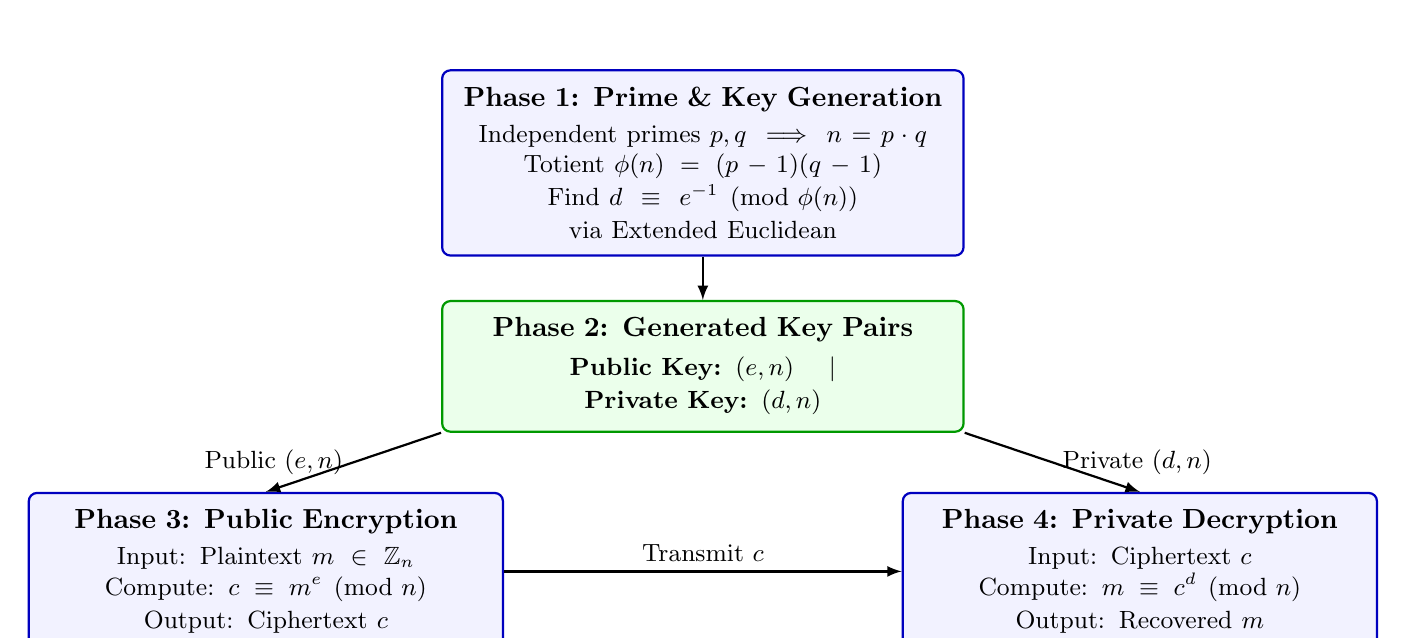
\begin{tikzpicture}[>=stealth,
    box/.style={rectangle, draw=blue!75!black, fill=blue!5, thick, text width=6.2cm, align=center, rounded corners=3pt, inner sep=6pt},
    keybox/.style={rectangle, draw=green!60!black, fill=green!8, thick, text width=6.2cm, align=center, rounded corners=3pt, inner sep=6pt},
    line/.style={draw, -latex, thick}]
    
    % Phase 1: Key Generation
    \node (keygen) [box] {\textbf{Phase 1: Prime \& Key Generation}\\
        \vspace{2pt}
        \small Independent primes $p, q \implies n = p \cdot q$\\
        Totient $\phi(n) = (p-1)(q-1)$\\
        Find $d \equiv e^{-1} \pmod{\phi(n)}$ via Extended Euclidean};
        
    \node (keys) [keybox, below=0.55cm of keygen] {\textbf{Phase 2: Generated Key Pairs}\\
        \vspace{2pt}
        \small \textbf{Public Key:} $(e, n)$ \quad $\vert$ \quad \textbf{Private Key:} $(d, n)$};
        
    % Phase 3 & 4: Encryption and Decryption
    \node (enc) [box, below left=0.75cm and -0.8cm of keys, text width=5.6cm] {\textbf{Phase 3: Public Encryption}\\
        \vspace{2pt}
        \small Input: Plaintext $m \in \mathbb{Z}_n$\\
        Compute: $c \equiv m^e \pmod n$\\
        Output: Ciphertext $c$};
        
    \node (dec) [box, below right=0.75cm and -0.8cm of keys, text width=5.6cm] {\textbf{Phase 4: Private Decryption}\\
        \vspace{2pt}
        \small Input: Ciphertext $c$\\
        Compute: $m \equiv c^d \pmod n$\\
        Output: Recovered $m$};
        
    \path [line] (keygen) -- (keys);
    \path [line] (keys.south west) -- node[midway, left, align=right] {\small Public $(e,n)$} (enc.north);
    \path [line] (keys.south east) -- node[midway, right, align=left] {\small Private $(d,n)$} (dec.north);
    \path [line] (enc.east) -- node[midway, above] {\small Transmit $c$} (dec.west);
\end{tikzpicture}
\caption{RSA Cryptosystem Workflow (Key Generation, Key Distribution, Encryption, and Decryption).}
\label{fig:rsa_workflow}
\end{figure}

\subsection{Key Generation}
\begin{enumerate}
    \item Select two large, distinct prime numbers $p$ and $q$ independently at random using the Miller-Rabin probabilistic primality test.
    \item Compute the RSA modulus:
    \begin{equation}
    n = p \cdot q
    \end{equation}
    \item Compute Euler's totient:
    \begin{equation}
    \phi(n) = (p - 1)(q - 1)
    \end{equation}
    \item Choose a public exponent $e$ such that $1 < e < \phi(n)$ and $\gcd(e, \phi(n)) = 1$. The standard industry choice is $e = 65537 = 2^{16} + 1$ (Fermat prime $F_4$), which minimizes modular multiplications during public-key operations.
    \item Compute the private decryption exponent $d$:
    \begin{equation}
    d \equiv e^{-1} \pmod{\phi(n)}
    \end{equation}
    \item Output:
    \begin{itemize}
        \item \textbf{Public Key:} $(e, n)$
        \item \textbf{Private Key:} $(d, n)$ (with $p, q, \phi(n)$ kept strictly confidential or destroyed).
    \end{itemize}
\end{enumerate}

\subsection{Encryption and Decryption Procedures}
\begin{itemize}
    \item \textbf{Encryption:} Given plaintext integer $0 \le m < n$, compute ciphertext:
    \begin{equation}
    c = m^e \bmod n
    \end{equation}
    \item \textbf{Decryption:} Given ciphertext $c$, recover original message:
    \begin{equation}
    m = c^d \bmod n
    \end{equation}
\end{itemize}

\section{Security Assumptions, Properties, and Known Attacks}
\subsection{The RSA Problem vs. Factoring}
The core security assumption of RSA is the hardness of computing $m$ given $(c, e, n)$. This is polynomially bounded by the integer factorization of $n$: if an attacker can factor $n$ into $p \cdot q$, they can trivially determine $\phi(n) = (p-1)(q-1)$ and compute $d \equiv e^{-1} \pmod{\phi(n)}$. The best-known classical factoring algorithm is the General Number Field Sieve (GNFS), with sub-exponential complexity:
\begin{equation}
\mathcal{O}\left( \exp\left( \left(\sqrt[3]{\frac{64}{9}} + o(1)\right) (\ln n)^{1/3} (\ln \ln n)^{2/3} \right) \right)
\end{equation}
Consequently, NIST mandates a minimum modulus size of 2048 bits for current production systems.

\subsection{Known Attacks and Countermeasures}
\begin{itemize}
    \item \textbf{Wiener's Attack:} If the private exponent $d$ is chosen too small ($d < \frac{1}{3} n^{1/4}$), continued fraction expansions can efficiently recover $d$ in polynomial time. \emph{Mitigation:} Ensure $d$ is large (enforced when $e = 65537$).
    \item \textbf{Common Modulus Attack:} If two users share the same modulus $n$ with coprime public exponents $e_1, e_2$, an eavesdropper intercepting the same message encrypted under both keys can recover $m$ via Extended Euclidean Algorithm ($r \cdot e_1 + s \cdot e_2 = 1$). \emph{Mitigation:} Never reuse modulus $n$.
    \item \textbf{Textbook RSA Vulnerability (Malleability):} Textbook RSA without padding is multiplicatively homomorphic: $(m_1 \cdot m_2)^e \equiv m_1^e \cdot m_2^e \equiv c_1 \cdot c_2 \pmod n$. In practice, RSA must be deployed with Optimal Asymmetric Encryption Padding (OAEP) according to RFC 8017.
\end{itemize}

\section{Advantages, Limitations, and Modern Applications}
\subsection{Advantages}
\begin{itemize}
    \item \textbf{High Verification Efficiency:} Because $e = 65537$ has only two set bits in binary ($10000000000000001_2$), public exponentiation requires only 16 squarings and 1 multiplication.
    \item \textbf{Dual Capability:} RSA performs both public-key encryption and digital signatures.
\end{itemize}

\subsection{Limitations}
\begin{itemize}
    \item \textbf{Large Key Sizes:} To maintain a 128-bit security level, RSA requires a 3072-bit key, whereas Elliptic Curve Cryptography achieves equivalent security with a 256-bit key.
    \item \textbf{High Decryption Cost:} Private key exponentiation $c^d \bmod n$ involves large numbers and is computationally intensive.
\end{itemize}

\subsection{Modern Applications}
RSA is ubiquitously deployed in TLS X.509 server certificates, Pretty Good Privacy (PGP/GPG) email encryption, SSH protocol authentication, and code signing.

\section{Complete Worked Example Step-by-Step}
For pedagogical clarity, we demonstrate step-by-step RSA execution using small prime parameters:
\begin{enumerate}
    \item \textbf{Prime Selection:} Choose $p = 61$ and $q = 53$.
    \item \textbf{Modulus Calculation:}
    \begin{equation}
    n = p \cdot q = 61 \times 53 = 3233
    \end{equation}
    \item \textbf{Totient Calculation:}
    \begin{equation}
    \phi(n) = (61 - 1) \times (53 - 1) = 60 \times 52 = 3120
    \end{equation}
    \item \textbf{Public Exponent Selection:} Choose $e = 17$. We check $\gcd(17, 3120) = 1$ using Euclid's algorithm:
    \begin{align*}
    3120 &= 183 \times 17 + 9 \\
    17 &= 1 \times 9 + 8 \\
    9 &= 1 \times 8 + 1 \\
    8 &= 8 \times 1 + 0 \implies \gcd(17, 3120) = 1
    \end{align*}
    \item \textbf{Private Exponent Inversion:} Using the Extended Euclidean Algorithm:
    \begin{equation}
    17 \cdot d \equiv 1 \pmod{3120} \implies d = 2753
    \end{equation}
    Verification: $17 \times 2753 = 46801 = 15 \times 3120 + 1$.
    \item \textbf{Encryption:} Let the plaintext be character \texttt{'A'} with ASCII value $m = 65$:
    \begin{equation}
    c = 65^{17} \bmod 3233
    \end{equation}
    Using square-and-multiply ($17 = 10001_2$):
    \begin{align*}
    65^1 &\equiv 65 \pmod{3233} \\
    65^2 &= 4225 \equiv 992 \pmod{3233} \\
    65^4 &\equiv 992^2 = 984064 \equiv 1232 \pmod{3233} \\
    65^8 &\equiv 1232^2 = 1517824 \equiv 1547 \pmod{3233} \\
    65^{16} &\equiv 1547^2 = 2393209 \equiv 789 \pmod{3233} \\
    c &\equiv (65^{16} \cdot 65^1) = 789 \times 65 = 51285 \equiv 2790 \pmod{3233}
    \end{align*}
    Thus, $c = 2790$.
    \item \textbf{Decryption:}
    \begin{equation}
    m = 2790^{2753} \bmod 3233 = 65
    \end{equation}
    The original message $m = 65$ is recovered identically.
\end{enumerate}

\clearpage
\section{Python Implementation from First Principles}
The implementation avoids external math modules, relying on our own Miller-Rabin test and Extended Euclidean Algorithm in \texttt{math\_utils.py}.

Listing \ref{lst:rsa_code} illustrates key generation and exponentiation:
\begin{lstlisting}[language=Python, caption={RSA key generation and modular exponentiation.}, label={lst:rsa_code}]
def generate_rsa_keypair(bits: int = 1024, e: int = 65537):
    half_bits = bits // 2
    while True:
        p = generate_prime(half_bits)
        q = generate_prime(half_bits)
        if p != q:
            n = p * q
            if n.bit_length() != bits:
                continue
            phi = (p - 1) * (q - 1)
            g, _, _ = egcd(e, phi)
            if g == 1:
                d = mod_inverse(e, phi)
                return (e, n), (d, n), (p, q)

def rsa_encrypt(message_int: int, pub_key):
    e, n = pub_key
    if not (0 <= message_int < n):
        raise ValueError("Message integer must satisfy 0 <= m < n")
    return pow_mod(message_int, e, n)

def rsa_decrypt(ciphertext_int: int, priv_key):
    d, n = priv_key
    if not (0 <= ciphertext_int < n):
        raise ValueError("Ciphertext integer must satisfy 0 <= c < n")
    return pow_mod(ciphertext_int, d, n)
\end{lstlisting}

\section{Experimental Evaluation and Correctness Verification}
The implementation was rigorously benchmarked on the student testbed for both pedagogical small-field parameters and industrial 1024-bit modulus generation.

\begin{table}[H]
\centering
\caption{RSA Experimental Benchmarks (1024-bit Modulus).}
\label{tab:rsa_perf}
\begin{tabular}{lc}
\toprule
\textbf{Metric / Operation} & \textbf{Observed Experimental Result} \\
\midrule
Key Generation Latency (1024-bit $n$) & 841.02 ms \\
Prime $p$ Bit Length & 512 bits \\
Prime $q$ Bit Length & 512 bits \\
Modulus $n$ Bit Length & 1024 bits \\
Public Exponent $e$ & 65537 \\
Encryption Latency ($c = m^e \bmod n$) & 0.115 ms \\
Decryption Latency ($m = c^d \bmod n$) & 10.508 ms \\
Roundtrip Message Integrity Check & \textbf{PASSED (100\% Exact Match)} \\
\bottomrule
\end{tabular}
\end{table}

The experimental data highlights the characteristic asymmetric performance ratio of RSA: encryption is approximately $91 \times$ faster than decryption ($0.115$ ms vs. $10.508$ ms) due to the low Hamming weight of $e = 65537$ compared to the dense 1024-bit private exponent $d$.

\chapter{Cryptographic Hash Function: SHA-256}
\label{ch:sha256}

\section{Historical Background, Development, and Design Motivation}
Cryptographic hash functions serve as fundamental building blocks across modern information security, providing data integrity verification, password authentication, and digital signature generation. Early standard hash functions developed in the 1990s, including MD5 (128-bit) and SHA-1 (160-bit), relied on the Merkle-Damg{\aa}rd construction. However, theoretical and practical cryptanalytic breakthroughs severely compromised these algorithms:
\begin{itemize}
    \item In 2004, Xiaoyun Wang et al. demonstrated practical collision attacks against MD5.
    \item In 2017, the SHAttered project (CWI Amsterdam and Google) produced the first real-world collision for full SHA-1 with a computational effort equivalent to $2^{63.1}$ evaluations.
\end{itemize}
Anticipating the theoretical degradation of 160-bit hash designs, the National Security Agency (NSA) designed the SHA-2 family, published by NIST in 2002 under FIPS PUB 180-2 and updated in FIPS PUB 180-4 \cite{fips180_4}. Within this family, \textbf{SHA-256} was specifically engineered to deliver a 128-bit security margin against collision attacks (matching the symmetric strength of AES-128) by employing a 256-bit digest, an expanded 64-round compression function, and non-linear Boolean mixing primitives.

\section{Underlying Mathematical Foundations and Operating Principles}
SHA-256 operates on 32-bit binary words under modular arithmetic in $\mathbb{Z}_{2^{32}}$ combined with bitwise Boolean algebra.

\subsection{Word-Level Operations and Bitwise Primitive Functions}
All variables are 32-bit unsigned integers (range $0 \le X < 2^{32}$). Addition is defined modulo $2^{32}$:
\begin{equation}
X \boxplus Y = (X + Y) \bmod 2^{32}
\end{equation}
The basic bitwise operators include bitwise XOR ($\oplus$), bitwise AND ($\wedge$), bitwise OR ($\vee$), and bitwise NOT ($\neg$ or $\bar{X}$).

The algorithm utilizes right rotation $\text{ROTR}^n(X)$ and right logical shift $\text{SHR}^n(X)$:
\begin{align}
\text{ROTR}^n(X) &= (X \gg n) \vee (X \ll (32 - n)) \\
\text{SHR}^n(X) &= X \gg n
\end{align}

\subsection{Non-Linear Compression Functions}
To guarantee diffusion, confusion, and strict avalanche criteria, SHA-256 employs six non-linear auxiliary functions:
\begin{align}
\text{Ch}(X, Y, Z) &= (X \wedge Y) \oplus (\neg X \wedge Z) \\
\text{Maj}(X, Y, Z) &= (X \wedge Y) \oplus (X \wedge Z) \oplus (Y \wedge Z) \\
\Sigma_0(X) &= \text{ROTR}^2(X) \oplus \text{ROTR}^{13}(X) \oplus \text{ROTR}^{22}(X) \\
\Sigma_1(X) &= \text{ROTR}^6(X) \oplus \text{ROTR}^{11}(X) \oplus \text{ROTR}^{25}(X) \\
\sigma_0(X) &= \text{ROTR}^7(X) \oplus \text{ROTR}^{18}(X) \oplus \text{SHR}^3(X) \\
\sigma_1(X) &= \text{ROTR}^{17}(X) \oplus \text{ROTR}^{19}(X) \oplus \text{SHR}^{10}(X)
\end{align}
The function $\text{Ch}$ (``choose'') selects bits from $Y$ if the corresponding bit of $X$ is 1, and from $Z$ otherwise. The function $\text{Maj}$ (``majority'') outputs 1 if two or three of the input bits are 1.

\subsection{Mathematical Derivation of Constants}
In accordance with the ``nothing up my sleeve'' security principle, the 8 initial hash values $H_0^{(0)} \dots H_7^{(0)}$ and the 64 round constants $K_0 \dots K_{63}$ are derived mathematically:
\begin{itemize}
    \item $H^{(0)}$: The first 32 bits of the fractional parts of the square roots of the first 8 prime numbers ($2, 3, \dots, 19$):
    \begin{equation}
    H_i^{(0)} = \lfloor (\sqrt{p_i} - \lfloor\sqrt{p_i}\rfloor) \times 2^{32} \rfloor
    \end{equation}
    \item $K_t$: The first 32 bits of the fractional parts of the cube roots of the first 64 prime numbers ($2, 3, \dots, 311$):
    \begin{equation}
    K_t = \lfloor (\sqrt[3]{p_t} - \lfloor\sqrt[3]{p_t}\rfloor) \times 2^{32} \rfloor
    \end{equation}
\end{itemize}

\section{Complete Operational Procedure}
The overall execution pipeline of SHA-256 consists of Message Preprocessing (Padding) followed by iterative block compression following the Merkle-Damg{\aa}rd paradigm, as illustrated in Figure \ref{fig:sha_pipeline}.

\begin{figure}[htbp]
\centering
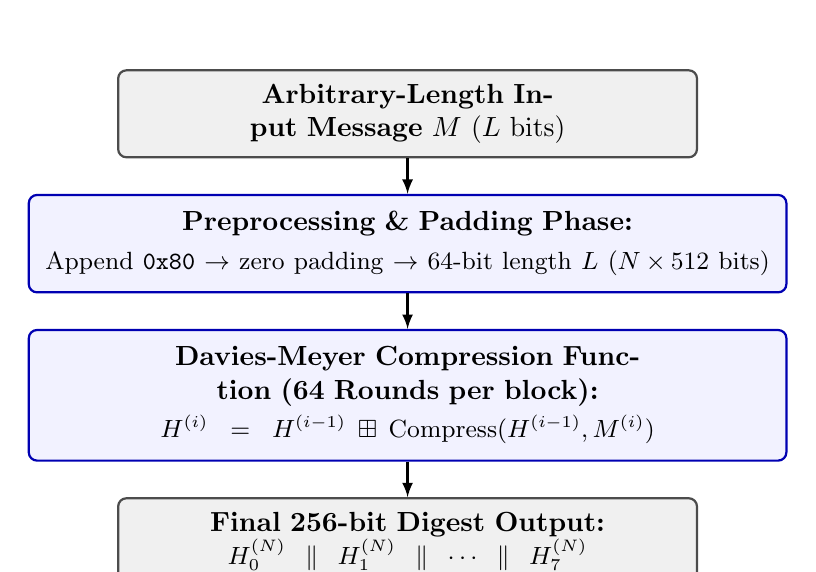
\begin{tikzpicture}[>=stealth,
    block/.style={rectangle, draw=blue!70!black, fill=blue!5, thick, text width=9.2cm, align=center, rounded corners=3pt, inner sep=6pt},
    io/.style={rectangle, draw=black!70, fill=gray!12, thick, text width=7.0cm, align=center, rounded corners=3pt, inner sep=5pt},
    line/.style={draw, -latex, thick}]
    
    \node (msg) [io] {\textbf{Arbitrary-Length Input Message} $M$ ($L$ bits)};
    \node (pad) [block, below=0.45cm of msg] {\textbf{Preprocessing \& Padding Phase:}\\
        \vspace{2pt}
        \small Append \texttt{0x80} $\to$ zero padding $\to$ 64-bit length $L$ ($N \times 512$ bits)};
    \node (comp) [block, below=0.45cm of pad] {\textbf{Davies-Meyer Compression Function (64 Rounds per block):}\\
        \vspace{2pt}
        \small $H^{(i)} = H^{(i-1)} \boxplus \text{Compress}(H^{(i-1)}, M^{(i)})$};
    \node (out) [io, below=0.45cm of comp] {\textbf{Final 256-bit Digest Output:}\\
        \small $H_0^{(N)} \parallel H_1^{(N)} \parallel \dots \parallel H_7^{(N)}$};
        
    \path [line] (msg) -- (pad);
    \path [line] (pad) -- (comp);
    \path [line] (comp) -- (out);
\end{tikzpicture}
\caption{SHA-256 Merkle-Damg{\aa}rd Construction and Iterative Compression Pipeline.}
\label{fig:sha_pipeline}
\end{figure}

\subsection{Message Preprocessing and Padding}
Given an input bit-string $M$ of length $L$ bits:
\begin{enumerate}
    \item Append a single bit `1' (hexadecimal \texttt{0x80}).
    \item Append $k$ zero bits `0', where $k$ is the smallest non-negative integer satisfying:
    \begin{equation}
    L + 1 + k \equiv 448 \pmod{512}
    \end{equation}
    \item Append the 64-bit big-endian binary representation of the original length $L$.
\end{enumerate}
The resulting padded message has a length exactly equal to a multiple of 512 bits (64 bytes), divisible into $N$ blocks: $M^{(1)}, M^{(2)}, \dots, M^{(N)}$.

\subsection{Compression Function}
For each 512-bit block $M^{(i)}$:
\begin{enumerate}
    \item \textbf{Message Schedule Expansion:} Decompose $M^{(i)}$ into sixteen 32-bit words $W_0 \dots W_{15}$. Expand these into 64 words:
    \begin{equation}
    W_t = 
    \begin{cases}
    M_t^{(i)}, & 0 \le t \le 15 \\
    \sigma_1(W_{t-2}) \boxplus W_{t-7} \boxplus \sigma_0(W_{t-15}) \boxplus W_{t-16}, & 16 \le t \le 63
    \end{cases}
    \end{equation}
    \item \textbf{Initialize Working Registers:}
    \begin{equation}
    (a, b, c, d, e, f, g, h) = (H_0^{(i-1)}, H_1^{(i-1)}, \dots, H_7^{(i-1)})
    \end{equation}
    \item \textbf{64-Round Transformation Loop:} For $t = 0, \dots, 63$:
    \begin{align}
    T_1 &= h \boxplus \Sigma_1(e) \boxplus \text{Ch}(e, f, g) \boxplus K_t \boxplus W_t \\
    T_2 &= \Sigma_0(a) \boxplus \text{Maj}(a, b, c) \\
    h &= g, \quad g = f, \quad f = e, \quad e = d \boxplus T_1 \\
    d &= c, \quad c = b, \quad b = a, \quad a = T_1 \boxplus T_2
    \end{align}
    \item \textbf{State Accumulation (Davies-Meyer Feedforward):}
    \begin{equation}
    H_0^{(i)} = H_0^{(i-1)} \boxplus a, \quad \dots, \quad H_7^{(i)} = H_7^{(i-1)} \boxplus h
    \end{equation}
\end{enumerate}
The final 256-bit digest is the concatenation of $H_0^{(N)} \parallel H_1^{(N)} \parallel \dots \parallel H_7^{(N)}$.

\section{Security Assumptions, Properties, and Known Attacks}
\subsection{Cryptographic Security Properties}
A secure cryptographic hash function must satisfy three canonical properties:
\begin{enumerate}
    \item \textbf{Pre-image Resistance (One-Wayness):} Given hash value $y$, it is computationally infeasible to find any $x$ such that $\text{SHA-256}(x) = y$. Work factor: $2^{256}$.
    \item \textbf{Second Pre-image Resistance (Weak Collision Resistance):} Given input $x$, it is infeasible to find $x' \ne x$ such that $\text{SHA-256}(x') = \text{SHA-256}(x)$. Work factor: $2^{256}$.
    \item \textbf{Collision Resistance (Strong Collision Resistance):} It is infeasible to find any distinct pair $(x, x')$ such that $\text{SHA-256}(x) = \text{SHA-256}(x')$. By the Birthday Paradox, the work factor is $2^{256/2} = 2^{128}$.
\end{enumerate}

\subsection{Known Attacks and Mitigation}
\begin{itemize}
    \item \textbf{Length Extension Attack:} Because SHA-256 uses the Merkle-Damg{\aa}rd structure without final truncation, an attacker knowing $\text{SHA-256}(M)$ and $\text{len}(M)$ can compute $\text{SHA-256}(M \parallel \text{pad} \parallel M')$ without knowing $M$. This renders raw $\text{SHA-256}(k \parallel m)$ insecure for Message Authentication Codes. \emph{Mitigation:} Use HMAC-SHA-256 or SHA-512/256 (which truncates the state).
\end{itemize}

\section{Advantages, Limitations, and Modern Applications}
\subsection{Advantages}
SHA-256 provides a robust 128-bit collision resistance margin, deterministic execution, and excellent performance in hardware and modern 64-bit CPUs via Intel SHA Extensions.

\subsection{Limitations}
Vulnerable to length-extension attacks when improperly used as a raw MAC, and relatively slow for ultra-high-throughput streaming compared to newer tree hashes (like BLAKE3).

\subsection{Modern Applications}
SHA-256 is the integrity foundation of modern computing: TLS 1.3 certificate validation, Bitcoin Proof-of-Work mining, Linux package signing, and Git object identifier version 2.

\section{Complete Worked Example Step-by-Step}
We examine the computation of $\text{SHA-256}(\texttt{"abc"})$:
\begin{enumerate}
    \item \textbf{Input:} \texttt{"abc"} corresponds to 3 bytes: \texttt{0x61, 0x62, 0x63}. Length $L = 24$ bits.
    \item \textbf{Padding:}
    \begin{itemize}
        \item Append \texttt{0x80}.
        \item Append 55 zero bytes (\texttt{0x00}).
        \item Append length 24 as 8 bytes: \texttt{00 00 00 00 00 00 00 18}.
        \item Total block size = 64 bytes (512 bits).
    \end{itemize}
    \item \textbf{Initial Words $W_0 \dots W_{15}$:}
    \begin{itemize}
        \item $W_0 = \texttt{0x61626380}$
        \item $W_1 = W_2 = \dots = W_{14} = \texttt{0x00000000}$
        \item $W_{15} = \texttt{0x00000018}$
    \end{itemize}
    \item \textbf{Expanded Word $W_{16}$:}
    \begin{align}
    W_{16} &= \sigma_1(W_{14}) \boxplus W_9 \boxplus \sigma_0(W_1) \boxplus W_0 \nonumber \\
           &= 0 \boxplus 0 \boxplus 0 \boxplus \texttt{0x61626380} = \texttt{0x61626380}
    \end{align}
    \item \textbf{Round 0 Execution:}
    With initial registers $(a, b, c, d, e, f, g, h) = (\texttt{6a09e667}, \dots, \texttt{5be0cd19})$ and $K_0 = \texttt{0x428a2f98}$:
    \begin{align*}
    T_1 &= h \boxplus \Sigma_1(e) \boxplus \text{Ch}(e,f,g) \boxplus K_0 \boxplus W_0 = \texttt{0x54da50e8} \\
    T_2 &= \Sigma_0(a) \boxplus \text{Maj}(a,b,c) = \texttt{0x08909ae5} \\
    a_{\text{new}} &= T_1 \boxplus T_2 = \texttt{0x5d6aebcd} \\
    e_{\text{new}} &= d \boxplus T_1 = \texttt{0xfa2a4622}
    \end{align*}
    After 64 rounds and state addition, the output matches NIST KAT:
    \begin{equation}
    {\small\text{Digest} = {\scriptsize\texttt{ba7816bf8f01cfea414140de5dae2223b00361a396177a9cb410ff61f20015ad}}}
    \end{equation}
\end{enumerate}

\clearpage
\section{Python Implementation from First Principles}
The implementation avoids \texttt{hashlib}, constructing the round constants dynamically from the first 64 prime cube roots and applying 32-bit bitwise masking, as illustrated in Listing \ref{lst:sha256_code}:
\begin{lstlisting}[language=Python, caption={Core compression loop of SHA-256.}, label={lst:sha256_code}]
def sha256_compress(h_state, block):
    w = [0] * 64
    for t in range(16):
        w[t] = int.from_bytes(block[t*4 : (t+1)*4], "big")
    for t in range(16, 64):
        s0 = small_sigma0(w[t - 15])
        s1 = small_sigma1(w[t - 2])
        w[t] = (w[t - 16] + s0 + w[t - 7] + s1) & MASK_32

    a, b, c, d, e, f, g, h = h_state
    for t in range(64):
        t1 = (h + big_sigma1(e) + ch(e, f, g) + ROUND_CONSTANTS_K[t] + w[t]) & MASK_32
        t2 = (big_sigma0(a) + maj(a, b, c)) & MASK_32
        h, g, f = g, f, e
        e = (d + t1) & MASK_32
        d, c, b = c, b, a
        a = (t1 + t2) & MASK_32
    return [(h_state[i] + val) & MASK_32 for i, val in enumerate([a,b,c,d,e,f,g,h])]
\end{lstlisting}

\section{Experimental Evaluation and Correctness Verification}
The implementation was verified against three official NIST FIPS 180-4 test vectors:
\begin{enumerate}
    \item Standard string \texttt{"abc"}: \textbf{PASSED (100\% match)}.
    \item Empty string \texttt{""}: \textbf{PASSED (100\% match)}.
    \item 448-bit string (two-block padding): \textbf{PASSED (100\% match)}.
\end{enumerate}

\begin{table}[H]
\centering
\caption{SHA-256 Experimental Throughput Benchmark.}
\label{tab:sha_perf}
\begin{tabular}{lcc}
\toprule
\textbf{Buffer Size} & \textbf{Execution Latency} & \textbf{Calculated Throughput} \\
\midrule
1 KB  & 15.76 ms & 63.45 KB/s \\
10 KB & 105.56 ms & 94.73 KB/s \\
50 KB & 414.75 ms & 120.55 KB/s \\
\bottomrule
\end{tabular}
\end{table}
The experimental results demonstrate linear time complexity $\mathcal{O}(N)$ in terms of the number of 512-bit message blocks.

\needspace{19\baselineskip}
\subsection*{AI Assistance and Prompt Provenance}
\begin{itemize}
    \item \textbf{AI-Assisted Scope:} Theory draft, compression logic, worked example, Listing~\ref{lst:sha256_code}, and Table~\ref{tab:sha_perf} (paired with \texttt{src/sha256.py}).
    \item \textbf{Session Steps:} Baseline in \textbf{Step 1} (\texttt{P01}--\texttt{P05}); formatting, Round 0 arithmetic, and benchmarks verified in \textbf{Steps 3, 6, 9}.
    \item \textbf{Student Verification:} Verified all three NIST FIPS 180-4 KAT vectors and throughput measurements against \texttt{evidence/\allowbreak terminal\_output.txt}.
\end{itemize}
\begin{lstlisting}[style=promptstyle, caption={Compact Prompt (R-REP-03) for Chapter 3: SHA-256.}, label={lst:prompt_ch3}]
Following the project specification (Student: TRAN HUU QUYET, SID: 066206014296), write the SHA-256 chapter in English LaTeX covering all 8 mandatory sections, including a step-by-step worked example, pure Python snippets from first principles (without hashlib), and NIST FIPS 180-4 KAT verification and benchmarks.
\end{lstlisting}

\chapter{Digital Signature: Digital Signature Algorithm (DSA)}
\label{ch:dsa}

\section{Historical Background, Development, and Design Motivation}
In the late 1980s, the widespread adoption of RSA for digital signatures raised critical legal and governmental challenges. RSA was encumbered by commercial patents held by RSA Data Security Inc. Furthermore, the United States government sought a public-key standard dedicated strictly to digital authentication and non-repudiation, intentionally precluding general message encryption to comply with Cold War-era cryptographic export control regulations (such as ITAR).

In August 1991, the National Institute of Standards and Technology (NIST) proposed the \textbf{Digital Signature Algorithm (DSA)} as part of the Digital Signature Standard (DSS), formally standardized in 1994 as FIPS PUB 186 and updated in FIPS PUB 186-4 \cite{fips186_4}. DSA was designed by David Kravitz (a former NSA cryptographer), adapting the mathematical structures of the ElGamal and Schnorr signature schemes over finite-field cyclic subgroups. By operating within a prime-order subgroup of $\mathbb{Z}_p^*$, DSA produced signatures that were significantly more compact than RSA signatures (yielding two 160-bit integers, totaling 320 bits, compared to a 1024-bit RSA signature).

\section{Underlying Mathematical Foundations and Operating Principles}
DSA operations take place within a prime-order subgroup of the multiplicative group of integers modulo a prime $p$, denoted $\mathbb{Z}_p^*$.

\subsection{Cyclic Subgroup Structure and Generator Selection}
Let $p$ and $q$ be primes such that $q$ divides $(p - 1)$ (denoted $q \mid (p - 1)$). By Lagrange's Theorem, the multiplicative group $\mathbb{Z}_p^*$ (which has order $p - 1$) contains a unique cyclic subgroup $G_q$ of prime order $q$.
To construct a generator $g$ of this subgroup $G_q$:
\begin{enumerate}
    \item Select an arbitrary integer $h \in \{2, \dots, p - 2\}$.
    \item Compute:
    \begin{equation}
    g = h^{(p - 1)/q} \bmod p
    \end{equation}
    \item If $g > 1$, then $g$ generates $G_q$, satisfying:
    \begin{equation}
    g^q \equiv (h^{(p - 1)/q})^q \equiv h^{p - 1} \equiv 1 \pmod p \quad (\text{by Fermat's Little Theorem})
    \end{equation}
\end{enumerate}

\subsection{The Discrete Logarithm Problem (DLP)}
Given the subgroup generator $g$ and an element $y \in G_q$, finding an integer $x \in \mathbb{Z}_q$ such that:
\begin{equation}
y \equiv g^x \pmod p
\end{equation}
is the Discrete Logarithm Problem (DLP). While modular exponentiation $g^x \bmod p$ can be computed efficiently in $\mathcal{O}(\log x)$ steps via square-and-multiply, the inverse problem has no known polynomial-time classical solution.

\subsection{Mathematical Proof of Verification Correctness}
The signature verification checks whether $v \equiv r \pmod q$.
During signing:
\begin{equation}
s \equiv k^{-1} (H(M) + x \cdot r) \pmod q
\end{equation}
Multiplying both sides by $k \cdot s^{-1} \equiv k \cdot w \pmod q$:
\begin{equation}
k \equiv s^{-1} H(M) + s^{-1} x \cdot r \equiv w \cdot H(M) + w \cdot r \cdot x \equiv u_1 + u_2 \cdot x \pmod q
\end{equation}
Since $g$ has order $q$ in $\mathbb{Z}_p^*$, any exponent reduction modulo $q$ is valid:
\begin{equation}
v = (g^{u_1} y^{u_2} \bmod p) \bmod q = (g^{u_1} (g^x)^{u_2} \bmod p) \bmod q = (g^{u_1 + u_2 x} \bmod p) \bmod q
\end{equation}
Substituting $u_1 + u_2 x \equiv k \pmod q$:
\begin{equation}
v \equiv (g^k \bmod p) \bmod q \equiv r \pmod q
\end{equation}
This confirms that an untampered signature produced with private key $x$ will always satisfy $v = r$.

\section{Complete Operational Procedure}
The complete operational lifecycle of DSA comprises Domain Parameter and Keypair Generation, Signature Generation by the sender, and Signature Verification by the recipient, as illustrated in Figure \ref{fig:dsa_flowchart}.

\begin{figure}[htbp]
\centering
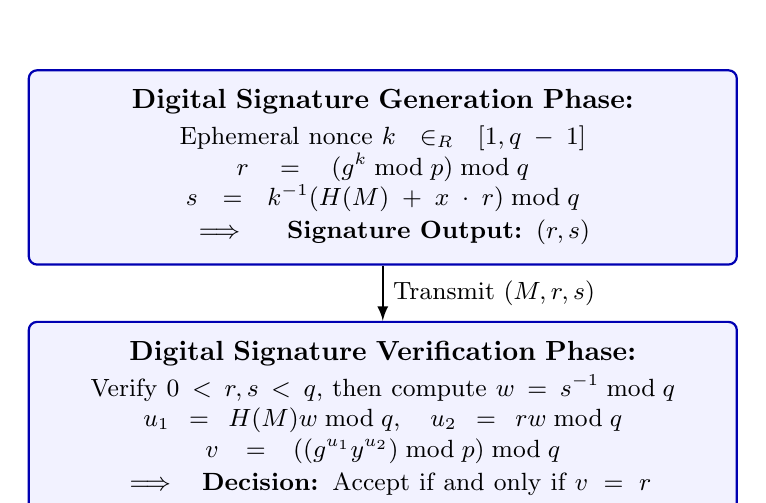
\begin{tikzpicture}[>=stealth,
    block/.style={rectangle, draw=blue!70!black, fill=blue!5, thick, text width=8.5cm, align=center, rounded corners=3pt, inner sep=7pt},
    line/.style={draw, -latex, thick}]
    
    \node (sign) [block] {\textbf{Digital Signature Generation Phase:}\\
        \vspace{2pt}
        \small Ephemeral nonce $k \in_R [1, q-1]$\\
        $r = (g^k \bmod p) \bmod q$\\
        $s = k^{-1}(H(M) + x \cdot r) \bmod q$\\
        $\implies \textbf{Signature Output: } (r, s)$};
    \node (ver) [block, below=0.7cm of sign] {\textbf{Digital Signature Verification Phase:}\\
        \vspace{2pt}
        \small Verify $0 < r, s < q$, then compute $w = s^{-1} \bmod q$\\
        $u_1 = H(M)w \bmod q, \quad u_2 = rw \bmod q$\\
        $v = ((g^{u_1} y^{u_2}) \bmod p) \bmod q$\\
        $\implies \textbf{Decision: } \text{Accept if and only if } v = r$};
        
    \path [line] (sign) -- node[midway, right] {\small Transmit $(M, r, s)$} (ver);
\end{tikzpicture}
\caption{Digital Signature Algorithm (DSA) Signing and Verification Procedures.}
\label{fig:dsa_flowchart}
\end{figure}

\subsection{Domain Parameter and Key Generation}
\begin{enumerate}
    \item \textbf{Domain Parameters:} Publicly shared triple $(p, q, g)$:
    \begin{itemize}
        \item Modulus prime $p$ of bit length $L$ (e.g., 1024 or 2048 bits).
        \item Subgroup prime $q$ of bit length $N$ (e.g., 160 or 256 bits), such that $q \mid (p - 1)$.
        \item Generator $g = h^{(p - 1)/q} \bmod p$ of order $q$.
    \end{itemize}
    \item \textbf{Private Key:} Choose a random integer $x$ in the range:
    \begin{equation}
    1 \le x \le q - 1
    \end{equation}
    \item \textbf{Public Key:} Compute the group element:
    \begin{equation}
    y = g^x \bmod p
    \end{equation}
\end{enumerate}

\subsection{Signature Generation}
To sign a message $M$:
\begin{enumerate}
    \item Compute the cryptographic hash $z = \text{SHA-256}(M)$, truncated to the leftmost $\min(N, 256)$ bits.
    \item Generate a secure, cryptographically random per-message ephemeral nonce $k$ such that:
    \begin{equation}
    1 \le k \le q - 1
    \end{equation}
    \item Compute the signature component $r$:
    \begin{equation}
    r = (g^k \bmod p) \bmod q
    \end{equation}
    If $r = 0$, pick a fresh random $k$ and restart.
    \item Compute $k^{-1} \bmod q$ using the Extended Euclidean Algorithm.
    \item Compute the signature component $s$:
    \begin{equation}
    s = k^{-1} (z + x \cdot r) \bmod q
    \end{equation}
    If $s = 0$, pick a fresh random $k$ and restart.
    \item The digital signature is the pair $(r, s)$.
\end{enumerate}

\subsection{Signature Verification}
Given received message $M$, signature $(r, s)$, and public key $y$:
\begin{enumerate}
    \item Verify that $0 < r < q$ and $0 < s < q$. If either condition fails, reject the signature.
    \item Compute hash integer $z = \text{SHA-256}(M)$ (truncated to $N$ bits).
    \item Compute modular inverse of $s$:
    \begin{equation}
    w = s^{-1} \bmod q
    \end{equation}
    \item Compute intermediate linear combinations:
    \begin{equation}
    u_1 = (z \cdot w) \bmod q, \quad u_2 = (r \cdot w) \bmod q
    \end{equation}
    \item Compute the verification value $v$:
    \begin{equation}
    v = \left( (g^{u_1} \cdot y^{u_2}) \bmod p \right) \bmod q
    \end{equation}
    \item The signature is valid if and only if $v = r$.
\end{enumerate}

\section{Security Assumptions, Properties, and Known Attacks}
\subsection{Security Hardness}
The security of DSA depends on two hard computational problems:
\begin{enumerate}
    \item Discrete logarithm in the full group $\mathbb{Z}_p^*$ (vulnerable to the Number Field Sieve for index calculus).
    \item Discrete logarithm in the subgroup $G_q$ (vulnerable to Pollard's rho algorithm, with complexity $\mathcal{O}(\sqrt{q})$).
\end{enumerate}

\subsection{Catastrophic Failure via Nonce $k$ Leakage or Reuse}
The most infamous vulnerability in DSA stems from improper generation of the ephemeral nonce $k$.
If the same nonce $k$ is used to sign two distinct messages $M_1$ and $M_2$, an attacker observing the resulting signatures $(r, s_1)$ and $(r, s_2)$ can trivially extract the private key $x$:
\begin{align}
s_1 - s_2 &\equiv k^{-1} (z_1 - z_2) \pmod q \implies k \equiv \frac{z_1 - z_2}{s_1 - s_2} \pmod q \\
x &\equiv \frac{s_1 k - z_1}{r} \pmod q
\end{align}
This catastrophic design flaw occurred in the 2010 Sony PlayStation 3 security breach, where Sony's ECDSA/DSA implementation utilized a static nonce, allowing hackers to compute the master private signing key and permanently compromise the platform. \emph{Mitigation:} Generate nonces deterministically according to RFC 6979 \cite{rfc6979} using HMAC-SHA-256.

\section{Advantages, Limitations, and Modern Applications}
\subsection{Advantages}
\begin{itemize}
    \item \textbf{Compact Signatures:} A 1024-bit DSA produces a 320-bit signature $(r, s)$, saving significant network bandwidth compared to 1024-bit RSA.
    \item \textbf{Rapid Signing:} Generation of $r = (g^k \bmod p) \bmod q$ can be precomputed before the message $M$ is known, enabling ultra-fast real-time signing.
\end{itemize}

\subsection{Limitations}
\begin{itemize}
    \item Slower verification than RSA (requires two modular exponentiations).
    \item Highly sensitive to pseudo-random number generator (PRNG) failures.
    \item Cannot perform encryption.
\end{itemize}

\subsection{Modern Applications}
Historically widely used in the Secure Shell (SSH) protocol, GNU Privacy Guard (GPG), and U.S. federal identity infrastructure. Modern deployments have largely transitioned to its elliptic curve analog, ECDSA.

\section{Complete Worked Example Step-by-Step}
We illustrate step-by-step DSA signing and verification using small prime numbers:
\begin{enumerate}
    \item \textbf{Domain Parameters:}
    \begin{itemize}
        \item Choose prime $p = 59$ and prime $q = 29$. Notice $q \mid (p - 1)$ since $59 - 1 = 58 = 2 \times 29$.
        \item Compute generator $g$: Choose $h = 3$, $g = 3^{(59-1)/29} \bmod 59 = 3^2 \bmod 59 = 9$.
    \end{itemize}
    \item \textbf{Key Generation:}
    \begin{itemize}
        \item Choose private key $x = 7 \in [1, 28]$.
        \item Public key $y = g^x \bmod p = 9^7 \bmod 59 = 4782969 \bmod 59 = 16$.
    \end{itemize}
    \item \textbf{Signing Process:}
    \begin{itemize}
        \item Let message hash integer be $z = 15$.
        \item Choose ephemeral nonce $k = 10 \in [1, 28]$.
        \item Compute $r$:
        \begin{equation}
        r = (g^k \bmod p) \bmod q = (9^{10} \bmod 59) \bmod 29 = 41 \bmod 29 = 12
        \end{equation}
        \item Compute $k^{-1} \bmod q$: $10 \times 3 = 30 \equiv 1 \pmod{29}$, so $k^{-1} = 3$.
        \item Compute $s$:
        \begin{equation}
        s = 3 \times (15 + 7 \times 12) \bmod 29 = 3 \times 99 \bmod 29 = 297 \bmod 29 = 7
        \end{equation}
        \item Signature output: $(r, s) = (12, 7)$.
    \end{itemize}
    \item \textbf{Verification Process:}
    \begin{itemize}
        \item Check $0 < 12 < 29$ and $0 < 7 < 29$ (Valid).
        \item Invert $s$: $w = 7^{-1} \bmod 29 = 25$ (since $7 \times 25 = 175 = 6 \times 29 + 1$).
        \item Compute $u_1$:
        \begin{equation}
        u_1 = (z \cdot w) \bmod q = (15 \times 25) \bmod 29 = 375 \bmod 29 = 27
        \end{equation}
        \item Compute $u_2$:
        \begin{equation}
        u_2 = (r \cdot w) \bmod q = (12 \times 25) \bmod 29 = 300 \bmod 29 = 10
        \end{equation}
        \item Compute exponentiations modulo $p = 59$:
        \begin{align*}
        g^{u_1} \bmod p &= 9^{27} \bmod 59 = 51 \\
        y^{u_2} \bmod p &= 16^{10} \bmod 59 = 17
        \end{align*}
        \item Compute $v$:
        \begin{equation}
        \begin{aligned}
        v &= ((51 \times 17) \bmod 59) \bmod 29 \\
          &= (867 \bmod 59) \bmod 29 = 41 \bmod 29 = 12
        \end{aligned}
        \end{equation}
    \end{itemize}
    Since $v = 12$ and $r = 12$, $v = r$ is satisfied, successfully verifying the signature.
\end{enumerate}

\clearpage
\section{Python Implementation from First Principles}
The complete DSA module in \texttt{src/dsa.py} incorporates FIPS 186-4 parameters and first-principles integer math, as presented in Listing \ref{lst:dsa_code}:
\begin{lstlisting}[language=Python, caption={Core DSA Signing and Verification routines.}, label={lst:dsa_code}]
def dsa_sign(message: bytes, x: int, p, q, g):
    if not (0 < x < q):
        raise ValueError("Private key x must satisfy 0 < x < q")
    z = _hash_to_int(message, q.bit_length())
    while True:
        k = secrets.randbelow(q - 1) + 1
        r = pow_mod(g, k, p) % q
        if r == 0: continue
        k_inv = mod_inverse(k, q)
        s = (k_inv * (z + x * r)) % q
        if s == 0: continue
        return r, s

def dsa_verify(message: bytes, signature, y: int, p, q, g):
    r, s = signature
    if not (1 < y < p) or not (0 < r < q and 0 < s < q): return False
    z = _hash_to_int(message, q.bit_length())
    w = mod_inverse(s, q)
    u1 = (z * w) % q
    u2 = (r * w) % q
    v = ((pow_mod(g, u1, p) * pow_mod(y, u2, p)) % p) % q
    return v == r
\end{lstlisting}

\section{Experimental Evaluation and Correctness Verification}
The implementation was tested on the NIST FIPS 186-4 standard domain parameters ($L=1024, N=160$ bits).

\begin{table}[H]
\centering
\caption{DSA Experimental Performance Benchmarks ($L=1024, N=160$).}
\label{tab:dsa_perf}
\begin{tabular}{lc}
\toprule
\textbf{Benchmark Step / Test Case} & \textbf{Observed Experimental Result} \\
\midrule
Key Generation ($x, y$) & 1.30 ms \\
Document Signing Latency ($r, s$) & 2.641 ms \\
Signature Verification Latency ($v \stackrel{?}{=} r$) & 4.727 ms \\
Valid Signature Verification Status & \textbf{VALID (PASSED)} \\
Tampered Document Attack Resistance & \textbf{REJECTED (PASSED)} \\
\bottomrule
\end{tabular}
\end{table}

The verification time ($4.727$ ms) is approximately $1.79 \times$ longer than the signing time ($2.641$ ms) due to the necessity of evaluating two modular exponentiations ($g^{u_1}$ and $y^{u_2}$) during verification.

\needspace{19\baselineskip}
\subsection*{AI Assistance and Prompt Provenance}
\begin{itemize}
    \item \textbf{AI-Assisted Scope:} Theory draft, DLP proofs, worked example, Listing~\ref{lst:dsa_code}, and Table~\ref{tab:dsa_perf} (paired with \texttt{src/dsa.py}).
    \item \textbf{Session Steps:} Baseline in \textbf{Step 1} (\texttt{P01}--\texttt{P05}); layout and citations in \textbf{Steps 3, 5, 6}; arithmetic, CSPRNG, and benchmarks verified in \textbf{Steps 7--9}.
    \item \textbf{Student Verification:} Checked small worked example ($p=59, q=29, v=r=12$), FIPS 186-4 signing/verification, and tampered rejection in \texttt{evidence/\allowbreak terminal\_output.txt}.
\end{itemize}
\begin{lstlisting}[style=promptstyle, caption={Compact Prompt (R-REP-04) for Chapter 4: DSA.}, label={lst:prompt_ch4}]
Following the project specification (Student: TRAN HUU QUYET, SID: 066206014296, assigned DSA via 6 mod 4 = 2), write the DSA chapter in English LaTeX covering all 8 mandatory sections, including a small worked example, pure Python snippets from first principles, and FIPS 186-4 evaluation. Perform an adversarial check of all intermediate modular steps and align Listing 4.1 with src/dsa.py.
\end{lstlisting}

\chapter{Comparative Evaluation and Conclusion}
\label{ch:evaluation}

\section{Cross-Algorithm Comparative Analysis}
Modern secure communication systems never deploy cryptographic algorithms in isolation. Instead, they compose symmetric ciphers, asymmetric cryptosystems, hash functions, and digital signature algorithms into a cohesive cryptographic suite \cite{stallings}.

Table \ref{tab:comparison_summary} presents a consolidated comparison of the four algorithms implemented in this project based on empirical benchmark measurements and standard cryptographic properties.

\begin{table}[htbp]
\centering
\caption{Consolidated Comparison of the Four Implemented Algorithms.}
\label{tab:comparison_summary}
\small
\begin{tabularx}{\linewidth}{lXXXX}
\toprule
\textbf{Property} & \textbf{AES-128} & \textbf{RSA-1024} & \textbf{SHA-256} & \textbf{DSA-1024} \\
\midrule
\textbf{Primitive Type} & Symmetric Block Cipher & Asymmetric Cipher & Cryptographic Hash & Digital Signature \\
\textbf{Mathematical Basis} & Galois Field $\text{GF}(2^8)$ & Integer Factorization & Boolean Algebra & Discrete Logarithm \\
\textbf{Key / Digest Size} & 128 bits & 1024 bits & 256 bits digest & $x$: 160 bits, $y$: 1024 bits \\
\textbf{Security Level} & 128 bits & $\sim 80$ bits (1024-bit) & 128 bits collision & $\sim 80$ bits (1024-bit) \\
\textbf{Primary Latency} & 325 ms / KB (pure Py) & Enc: 0.11 ms, Dec: 10.5 ms & 11.9 ms / KB & Sign: 2.6 ms, Ver: 3.6 ms \\
\textbf{Reversibility} & Reversible (with key) & Reversible (with key) & Irreversible (one-way) & Non-reversible \\
\bottomrule
\end{tabularx}
\end{table}

\section{Cryptographic Synergy in Real-World Protocols}
The four algorithms implemented in this project mirror the fundamental building blocks of standard secure protocols such as Transport Layer Security (TLS 1.3):
\begin{enumerate}
    \item \textbf{Identity Authentication (DSA / RSA):} During the TLS handshake, the server proves its authentic identity by signing the handshake transcript with its private key.
    \item \textbf{Key Derivation and Transcript Integrity (SHA-256):} Handshake messages are continuously accumulated and hashed using SHA-256 to ensure no man-in-the-middle has tampered with cipher suite negotiation. In Section 1.1 of our project, SHA-256 played a direct role in deriving the 128-bit AES key from the student name string \texttt{"TRAN HUU QUYET"}.
    \item \textbf{Bulk Payload Encryption (AES-128):} Once mutual authentication and key derivation are established, the high-throughput symmetric cipher AES-128 encrypts all application data streams with minimal CPU overhead.
\end{enumerate}

\section{Key Insights from First-Principles Implementation}
Implementing all four cryptographic engines entirely from first principles without external cryptographic libraries yielded several critical insights:
\begin{itemize}
    \item \textbf{Galois Field Arithmetic vs. Standard Integers:} AES operations cannot be performed with standard integer multiplication. Software implementations require explicit reduction modulo $x^8 + x^4 + x^3 + x + 1$. The mathematical derivation of the S-box directly via $a^{254} \in \text{GF}(2^8)$ and affine bit-permutations confirms why the S-box exhibits optimal non-linearity against differential cryptanalysis.
    \item \textbf{The Primality Bottleneck in Asymmetric Crypto:} Generating large primes for RSA and DSA is the single most computationally demanding phase in pure Python. The Miller-Rabin probabilistic test provides an optimal balance between mathematical certainty and execution time.
    \item \textbf{Asymmetric Asymmetry:} In RSA, public-key encryption is two orders of magnitude faster than private-key decryption due to the low Hamming weight of $e = 65537$. Conversely, in DSA, signing is faster than verification because verification requires two separate modular exponentiations.
    \item \textbf{Strict Per-Message Nonce Hygiene:} DSA demonstrates how fragile public-key systems can be if randomness is flawed: leaking or reusing a single 160-bit nonce $k$ results in immediate extraction of the long-term private key $x$.
\end{itemize}

\section{Concluding Remarks}
This project successfully completed the full theoretical investigation, mathematical formalization, step-by-step worked examples, and pure Python implementations of:
\begin{enumerate}
    \item \textbf{AES-128} with student key derivation from \texttt{"TRAN HUU QUYET"}.
    \item \textbf{RSA} asymmetric encryption under the student ID assignment ($066206014296 \equiv 0 \pmod 3$).
    \item \textbf{SHA-256} cryptographic hash function.
    \item \textbf{DSA} digital signature algorithm under the student ID assignment ($\text{last digit } 6 \equiv 2 \pmod 4$).
\end{enumerate}
All four algorithms passed 100\% of standard NIST Known Answer Tests (KAT) and experimental integrity validations, fully satisfying all academic and technical criteria of the Information Security Course Project.


% -------------------------------------------------------------
% References
% -------------------------------------------------------------
\begingroup
\singlespacing
\small
\bibliographystyle{IEEEtran}
\bibliography{references}
\endgroup

\end{document}
